\section*{Источники и решения}

\subsubsection*{Уже упал?}

Насколько мне известно, первая публикация этой замечательной головоломки состоялась в веб-колонке «Math Fun Facts» Фрэнсиса Су из Колледжа Харви Мадда \cite{math-fun-facts};
Фрэнсис припоминает, что услышал её в Европе от некого Феликса Варди, кого он не смог найти.
После этого головоломка появилась в журнале Emissary \cite[Весна/Осень 2003]{3}.

Дэн Амир, бывший ректор Тель-Авивского университета, увидел головоломку в Emissary и показал её тель-авивскому математику Ноге Алону, который привёз головоломку в принстонский Институт перспективных исследований;
я же услышал её от Ави Вигдерсона из этого института в конце 2003 года.

Ключ к этой и последующим головоломкам в том, что если бы муравьи были взаимозаменяемы, то было бы без разницы, проходят они сквозь друг друга или разворачиваются при встрече.
Тогда каждый муравей просто идёт прямо и должен упасть в течение 100 секунд.
Поскольку через 100 секунд упали все, то и Элис упал.

Если хочется избежать анонимности муравьёв, то можно думать, что каждый из них несёт флажок.
При встрече они обмениваются флажками и разворачиваются.
Таким образом, каждый муравей всегда несёт один флажок, а при встрече муравьёв флажки проходят мимо друг друга.
Если со стержня упали все флажки, то упали и муравьи.

Если начать с муравья, стоящего лицом на восток на западном конце шеста, то легко добиться того, чтоб к 100-й секунде Элис поднёс его флажок к восточному концу.
Поэтому 100 секунд ожидания необходимы и достаточны.

\subsubsection*{Элис на окружности}

Как и раньше, будем думать, что муравьи несут по флажку и обмениваются ими при встрече.
Тогда каждый флажок проходит полный круг за заданный период времени, заканчивая там, где начал.
При этом циклический порядок муравьёв не меняется, и значит (в большинстве случаев) произошёл циклический сдвиг.
То есть каждый муравей сдвинулся на определённое число позиций, скажем $k$, по часовой стрелке.
В частности, если Элис вернулся на своё место, то вернулись и все остальные.

Заметим, что если изначально $m$ муравьёв направлены по часовой стрелке, то в любой момент времени ровно $m$ муравьёв идут по часовой стрелке, и ровно $24 - m$ против.
Ведь при каждом столкновении муравей, движущийся по часовой стрелке, становится движущимся против часовой стрелки, и наоборот.
(Про это можно думать как о сохранении момента импульса!)
В любом случае, за время всего эксперимента один муравей сдвинется в среднем на $100(2m - 24)/24$ см по часовой стрелке.
Значит, каждый вернётся на своё место тогда и только тогда, когда $2m - 24$ кратно $24$; то есть, если $m = 0$, $24$ или $12$.

Первые два случая (когда все смотрят в одном направлении) имеют незначительную вероятность, но вклад последнего составляют внушительные $16{,}1180258\%$. %??? было неправильно 16,1180377 

Чтобы быть совсем точными, у нас есть $2^{24}=16\,777\,216$ вариантов выбрать направления, из которых  $\binom{24}0+\binom{24}{12}+\binom{24}{24}=1+2\,704\,156+1$ возвращают Элисa на место.
Это даёт вероятность $2\,704\,158/16\,777\,216 \z\sim 0{,}161180377$.

\subsubsection*{Какой конец?}

Заметим, что с восточного конца падают столько же муравьёв, сколько их смотрело на восток вначале.
Действительно, число муравьёв, смотрящих на восток, меняется только при падении муравья с воточного конца.
(Также можно думать об упавших со стержня флажках).
В любом случае, если $k$ муравьёв падают с восточного конца, то это происходит с $k$ самыми восточными муравьями, ведь их порядок на стержне не меняется.

Воспользовавшись симметрией, можно предположить, что вначале Элис смотрит на восток.
Как мы уже знаем, он упадёт с восточного конца, если вначале на восток смотрело $13$ или более муравьёв.
Это означает, что $12$ или более из оставшихся $24$-х смотрят на восток.
Вероятность того, что $13$ или более из $24$-х муравьёв смотрят на восток, такая же, как вероятность того, что $11$ или менее смотрят на восток, поэтому вероятность события, которое нас интересует, равна половинке плюс половине вероятности того, что ровно $12$ из $24$-х муравьёв смотрят на восток.

Последняя составляет $\binom{24}{12}/2^{24}$, что даёт $0{,}161180258$.
Получаем ответ $0{,}580590129\dots$, то есть чуть больше чем 58\%.

\subsubsection*{Кто последний?}

Можно предположить (снова используя симметрию), что Элис падает с восточного конца,
а значит и $12$ муравьёв к востоку от него делают то же самое.
Если он падает последним, то 12 муравьёв к западу от Элис упадут с западного конца.
То есть изначально ровно 12 флажков, а значит, и 12 муравьёв, повёрнуты на запад.
Это происходит с вероятностью $\binom{25}{12}/2^{24}$, то есть примерно в $31\%$ случаев.

Однако и в этом случае Элис не обязательно упадёт последним;
примерно в половине случаев эта честь достанется его западному соседу.
Таким образом, интересующая нас вероятность будет около $15{,}5\%$.

Но не стоит довольствоваться приближением если можно найти точный ответ.
Время, которое каждый флажок обречён провести на стержне, независимо и равномерно распределено между $0$ и $100$ секундами.
Таким образом, вероятность того, что самый долгоживущий флажок это один из 13 восточно-направленных флажков, составляет $13/25$.
Значит точный ответ $13/25 \z\times\binom{25}{12}/2^{24}$, и это уже знакомое нам число $\binom{24}{12}/2^{24}\sim 0{,}161180258$.

\subsubsection*{Число столкновений}

Каждый флажок встретится с каждым флажком расположенным впереди него и направленным к нему.
В среднем перед флажком стоит $12$ других и
половина из них (в среднем) направлена к нему.
Таким образом, флажок сталкивается с шестью другими, и всего $25 \times 6 = 150$ столкновений для всех флажков в среднем.
При этом каждое столкновение считается дважды, и ответ $75$.

А вот другой, немного более строгий способ вычисления:
Какова вероятность того, что два флажка столкнутся?
Независимо от их местоположения это происходит, только если они направлены друг к другу,
таким образом, вероятность $\tfrac14$.
По линейности матожидания число столкновений равно $\binom{25}2 \times \tfrac14 = 25 \times 24 /8 = 75$.

Кстати, максимальное число столкновений достигается, если все муравьи направлены к Элис (центральностоящему муравью).
В этом случае все $13$ флажков за Элисом сталкиваются со всеми $12$-ю флажками перед Элисом --- всего $12 \times 13 = 156$ столкновений.

Наименьшее возможное число столкновений, конечно, равно нулю, но это происходит с ничтожной вероятностью $26/2^{25} \sim 0{,}000000774860382$.


\subsubsection*{Помятость Элиса}

Легко подсчитать столкновения флажка Элиса.
Пусть Элис изначально смотрит на восток, в среднем $6$ из $12$ флажков перед Элисом, смотрят на запад.
Следовательно, в среднем  флажок Элиса столкнётся с шестью другими.

Но Элис не всегда несёт свой исходный флажок, и похоже, он сталкивается чаще других.
Почему?
Ну в среднем у муравья по шесть столкновений ($75 \z\times 2/25$), у крайних не больше одного, а у Элиса, стоящего посредине, должен быть больше среднего.

Заметим, что каждый муравей сталкивается только со своими двумя соседями,
и чередует их (ведь и его направление чередуется между столкновениями).
Последнее столкновение муравья будет с его западным соседом, если он свалится с восточного конца, и наоборот --- с его восточным соседом, если он свалится с западного конца.

Предположим, что вначале $k$ муравьёв смотрят на запад.
Поскольку их флажки идут к западному концу, $k$ самых западных муравьёв сваливаются с западного конца.
Тот из них, кто вначале смотрел на запад, имеет одинаковое число столкновений с обоих сторон;
тот же, кто смотрел на восток, имеет на одно столкновение больше с восточной стороны.
Таким образом, число столкновений между $j$-ым  (считая с запада) и 
$(j+1)$-ым муравьём равно числу, смотрящих на восток, среди муравьёв от $1$ до $j$ --- при условии, что $j\le k$.

В силу симметрии можно предположить, что $k$ находится между $13$ и $25$ (так, что Элис сваливается с западного конца).
Тогда число столкновений между Элис и его западным соседом равно числу муравьёв, смотрящих на восток, к западу от Элис; обозначим это число $x$.
Значит общее число столкновений Элиса будет равно $2x$ или $2x+1$ в зависимости от того, смотрел он на запад или восток вначале.

Априорное матожидание $\mathbb{E}[x]$ для $x$ равно $6$, так как западнее Элис $12$ муравьёв, каждый из которых может смотреть в любом направлении.
Однако мы только что предположили (чёрт!), что больше половины муравьёв смотрят на запад.
Но обратите внимание, что поскольку ожидаемое число муравьёв, смотрящих на восток, к востоку от Элис также равно $\mathbb{E}[x]$, число, которое мы ищем, является именно общим ожидаемым числом муравьёв, смотрящих на восток, даже учитывая, что они в меньшинстве.

Предположим, что муравьи были расставлены в алфавитном порядке, и последним стоял Яша.
Существует $2^{25}/2=2^{24}$ способа сделать такое распределение, чтобы получить большинство западных направлений и $\binom{24}{12}$
из них дают ровно $12$ муравьёв, направленных на восток, среди первых $24$ муравьёв.
В этом случае Яша обязан смотреть на запад,
а в остальных случаях он равновероятно смотрит на запад или на восток.
Следовательно, вероятность того, что Яша смотрит на восток, составляет
$0{,}419409871$.

Поскольку вероятность того, что Яша смотрит на восток, не отличается от этой же вероятности для любого другого муравья, умножив её на $25$, получим матожидание числа муравьёв, смотрящих на восток, что примерно $10{,}4852468$.
Именно это и является средним числом столкновений Элиса.

\subsubsection*{Страховой рейтинг Элиса}

Предположим, что самые западные $k$ муравьёв падают с западного конца,
а остальные с восточного.
Мы уже видели в предыдущем решении, что если $c_i$ --- число столкновений между $i$-ым (считая с западного конца) и $(i + 1)$-ым муравьём, то $c_i$ остаётся тем же или увеличивается на $1$ до $i = k$; после этого остаётся тем же или уменьшается на $1$.
В частности, $c_i=c_{i-1}$ ровно тогда, когда $i$-ый муравей смотрит (изначально) в том же направлении, с которого он упадёт.

Число столкновений $i$-го муравья равно $c_{i-1}+c_{i}$.
Значит, Элис обойдёт всех по числу столкновений, если $c_{11}+c_{12}\z<c_{12}\z+c_{13}\z>c_{13}\z+c_{14}$, а это значает, что  $c_{11}<c_{13}$ и $c_{12}>c_{14}$.
Это может произойти только если $c_{11}<c_{12}=c_{13}>c_{14}$, а значит, что $k = 12$ или $13$, и что Элис смотрит в том направлении, с которого падает,
и что оба его соседа смотрят в противоположные стороны от тех концов, с которых они падают.
Похоже, что это даёт вероятность 
\[\left(\tbinom{25}{12}+\tbinom{25}{12}\right)/2^{25}\cdot (\tfrac12)^3\sim 3.87452543\%,\]
однако эти события не совсем независимы.

Предположим, что Элис смотрит на восток, его восточный сосед --- Шурик, а западный сосед --- Юрик.
Шурик, как и Элис, будет падать с восточного конца и, следовательно, изначально должен был смотреть на запад (вероятность $1/2$).
Юрик --- один из $12$ муравьёв, падающих с западного конца и, следовательно, вначале он смотрел на восток (опять вероятность $1/2$).
Из оставшиеся 22 муравьёв половина должна смотреть на запад, а половина на восток (вероятность $\binom{22}{11}/2^{22}$), поэтому точный ответ составит
\[\left(\frac12\right)^2\cdot\binom{22}{11}/2^{22}\sim 4{,}20470238\%.\]

\subsubsection*{Насморк}

Эта головоломка чисто комбинаторная, как и многие другие в этой главе.
В частности, хоть это и не совсем очевидно, ответ не зависит от длины стержня.
Может показаться, что более короткий стержень позволит некоторым муравьям выбраться с него до того, как они успеют заразиться, однако как только муравей направляется к концу и перед ним нет других, его столкновениям пришёл конец.

Наверно, проще всего считать, что заражаются не муравьи, а флажки.
Мы можем предположить, что Элис смотрит на восток.
Тогда флажки, направленные на запад впереди него, встретят его флажок и заразятся.
В то же время флажки, направленные на восток впереди него, избегут заражения.
Тем временем флажки, направленные на запад, после встречи с флажком Элиса, заражают все флажки, направленные на восток позади Элиса, и в то же время флажки, направленные на запад позади Элис, избегут заражения.

Поскольку в среднем впереди Элиса находится 6 флажков, направленных на запад, и 6 флажков, направленных на восток, у нас 13 заражённых флажков (включая флажок Элиса) и, таким образом, всего 13 заражённых муравьёв в среднем.

Однако в наше рассуждение закралась небольшая ошибка: если впереди Элиса вовсе нет муравьёв, смотрящих на запад, то нет и флажка, который мог бы встретить флажок Элиса и заразить флажки, направленные на восток, позади него.
Такое происходит с вероятностью $1/2^{12}$ и уменьшает ожидаемое число заражённых с $7$ (Элис плюс в среднем 6 флажков, направленных на восток, позади него) до 1 (только Элис).
Таким образом, правильный ответ не $13$, а $13 - 6/2^{12} \sim 12{,}9985352$ заражённых муравьёв в среднем.

\subsubsection*{Элис посредине}

Джон Гилфорд из Agilent Technologies показал эту головоломку Стэну Вагону,
тот однажды осенью 2003 года объявил её «задачей недели» колледжа Макалестер.
Я узнал о задаче в январе 2004 года от Элвина Берлекэмпа на конференции «Joint Mathematics Meetings» в Финиксе.
Именно тогда главный герой этой главы получил своё имя;
думаю, что у Элвина на самом деле есть тётя Элис.
На меня ещё повлияло и присутствие на конференции издателя этой книги, Элис Питерс из A K Peters, Ltd.

Предположим, как обычно, что каждый муравей несёт флажок, и флажками обменивается при встрече.
Затем каждый флажок проходит ровно один метр, один раз отскакивая от конца и заканчивая свой путь в точке, симметричной его начальной позиции.
В частности, флажок Элис заканчивает свой путь снова в центре. Но будет ли Элис его нести?

Несоменно будет, потому что муравьи остались в исходном порядке.
$12$ флажков с западной стороны теперь находятся на восточной, и наоборот, так что у Элиса опять $13$-й флажок, и сам Элис всё ещё $13$-й с конца.

Таким образом, Элис оказывается там, где начал.
Другими словами, максимальное расстояние, на которое он может отойти от своей начальной точки, равно нулю.

\subsubsection*{Новое место Элиса}

Это вариация головоломки, придуманной Ногой Алоном и Одедом Маргалитом из Тель-Авивского университета, которую передал мне Нога.

Пусть $x_1,\dots,x_{12}$ --- начальные позиции $12$ муравьёв, обращённых на запад, пронумерованные с запада на восток.
Позиции задаются в сантиметрах от западного конца.
Положим, что $k$ таково, что флажки, стартовавшие с $x_k,\dots,x_{12}$, не упадут, и следовательно окажутся в позициях $x_k-63,\dots,x_{12}-63$.

Муравьи, конечно же, не меняют порядка на стержне.
Поскольку $k-1$ флажок упадёт с западного конца, Элис упадёт в случае если $k> 5$.
В противном случае он становится $(6-k)$-м оставшимся муравьём, считая с западного конца, что помещает его в позицию $x_{k+(5-k)}-63=x_5-63$.
Таким образом, всё, что вам нужно знать, это позиция 12-го муравья к востоку от Элиса, то есть $17$-го от западного конца.
Элис окажется на $63$ см к западу от этой точки;
если эта точка уже находится менее чем в $63$ см от западного конца, то Элис свалился.

\begin{figure}[ht!]
\centering
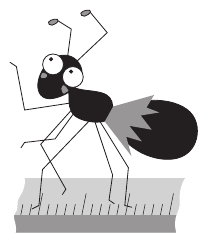
\includegraphics[scale=1]{pics/alice2}
\caption{Элис прощается.}
\label{pic:alice2}
\end{figure}
